\section{CINEMÁTICA}
\subsection{Parabólico Tradicional}
\begin{frame}{CINEMÁTICA}
	\framesubtitle{Parabólico Tradicional}
	\begin{equation}
	x\left( t \right)=-v_{0}\cos \theta t+x_{0}
	\end{equation}
    \begin{equation}
    y(t)=-\frac { 1 }{ 2 } g{ t }^{ 2 }+{ v }_{ 0 }\sin { \theta t+{ y }_{ 0 } }
    \end{equation}
    \begin{equation}
    y\left( x \right)=y_{0}+x\tan \theta -\frac{g}{2v_{0}^{2}\cos ^{2}\theta }x^2
    \end{equation}
	\begin{figure}[H]
  		\centering
  		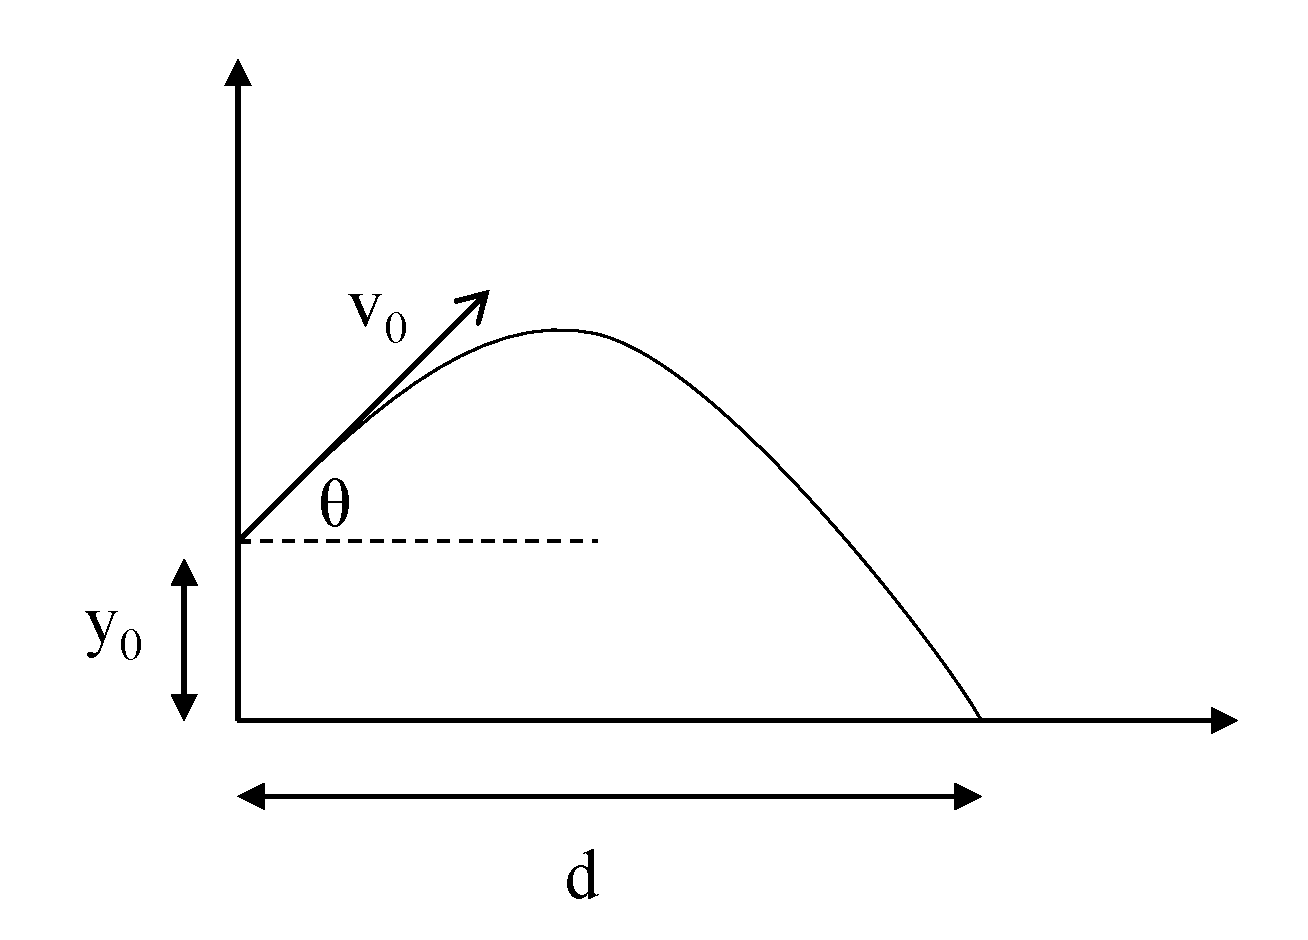
\includegraphics[scale = 0.2]{Motion.eps}
 		\caption{Movimiento parabólico.}
	\end{figure}
\end{frame}
%%%%%%%%%%%%%%%%%%%%%%%%%%
\subsection{Resistencia Simple al Aire}
\begin{frame}{CINEMÁTICA}
\framesubtitle{Resistencia Simple al Aire}
	\begin{equation}
    \begin{gathered}
	\Sigma F_y = -mg -kv_{y} = ma_y\\
    \Sigma F_x = -kv_{x} = ma_x
    \end{gathered}
	\end{equation}
	\begin{figure}[H]
  		\centering
  		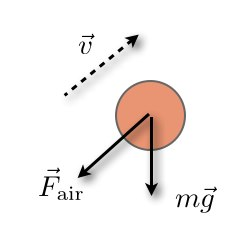
\includegraphics[scale = 0.4]{fbdBall.jpg}
 		\caption{Diagrama de cuerpo libre para una bola con resistencia simple al aire.}
	\end{figure}
\end{frame}
%%%%%%%%%%%%%%%%%%%%%%%%
\begin{frame}{CINEMÁTICA}
\framesubtitle{Resistencia Simple al Aire}
\begin{equation}
x\left( t \right)=x_{0}-\frac{v_{ox}m}{k}e^{-\frac{k}{m}t;}
\end{equation}
\begin{equation}
	y\left( t \right)=y_{0}-\frac{m}{k}\left[ gt+\left( v_{0y}+\frac{mg}{k} \right)e^{-\frac{k}{m}t} \right]
\end{equation}
\begin{equation}
	y\left( x \right)=\frac{m^{2}g}{k^{2}}\ln \left( -\frac{k}{mv_{0y}}x \right)+\left( 1+\frac{mg}{kv_{0x}} \right)
\end{equation}
	\begin{figure}[H]
  		\centering
  		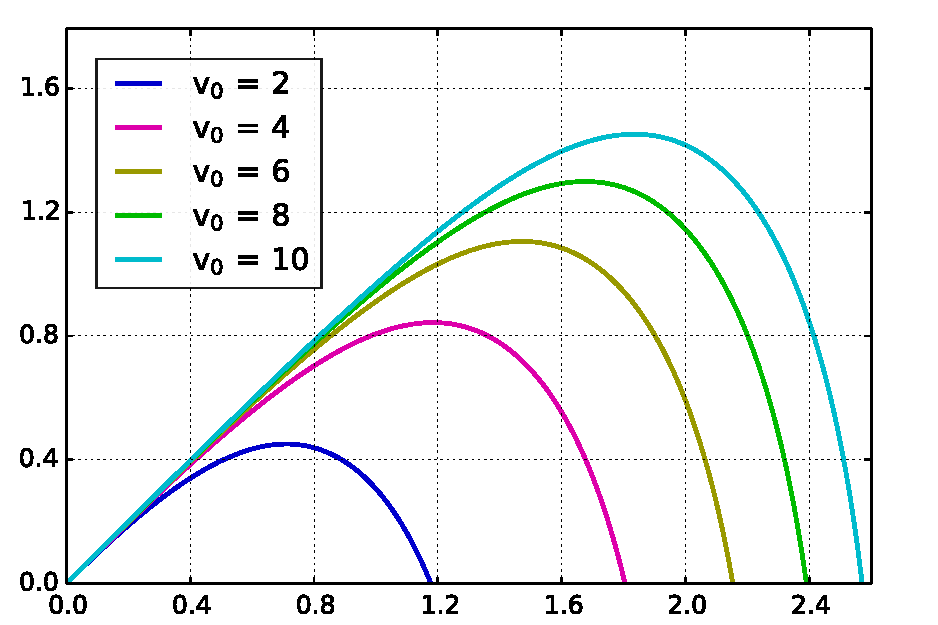
\includegraphics[scale = 0.3]{balistico.pdf}
 		\caption{Movimiento de un objeto con resistencia al aire para diferentes velocidades iniciales\footnotemark{}.}
	\end{figure}
    \vspace{-1cm}\footnotetext{\bibentry{airRes}}
    \footnotetext{Simulación: \url{https://www.geogebra.org/m/rYmNxYMY}}
\end{frame}

%%%%%%%%%%%%%%%%%%%%%%%%%%%%%%%%%%%%%%%%%%%%%%%%%
\subsection{Ecuación de Navier-Stokes}
\begin{frame}{CINEMÁTICA}
\framesubtitle{Ecuación de Navier-Stokes}
\url{https://www.youtube.com/watch?v=azyN4CXCiEE}
\begin{equation}
\rho \left( \frac{\partial u}{\partial t}+u\cdot\nabla\; u \right)=-\nabla\; p+\nabla\cdot\left( \mu \left( \nabla\; u\; +\; \left( \nabla\; u \right)^{T} \right)-\frac{2}{3}\mu \left( \nabla\cdot\; u \right)I \right)+\rho g+F
\end{equation}
	\begin{figure}[H]
  		\centering
  		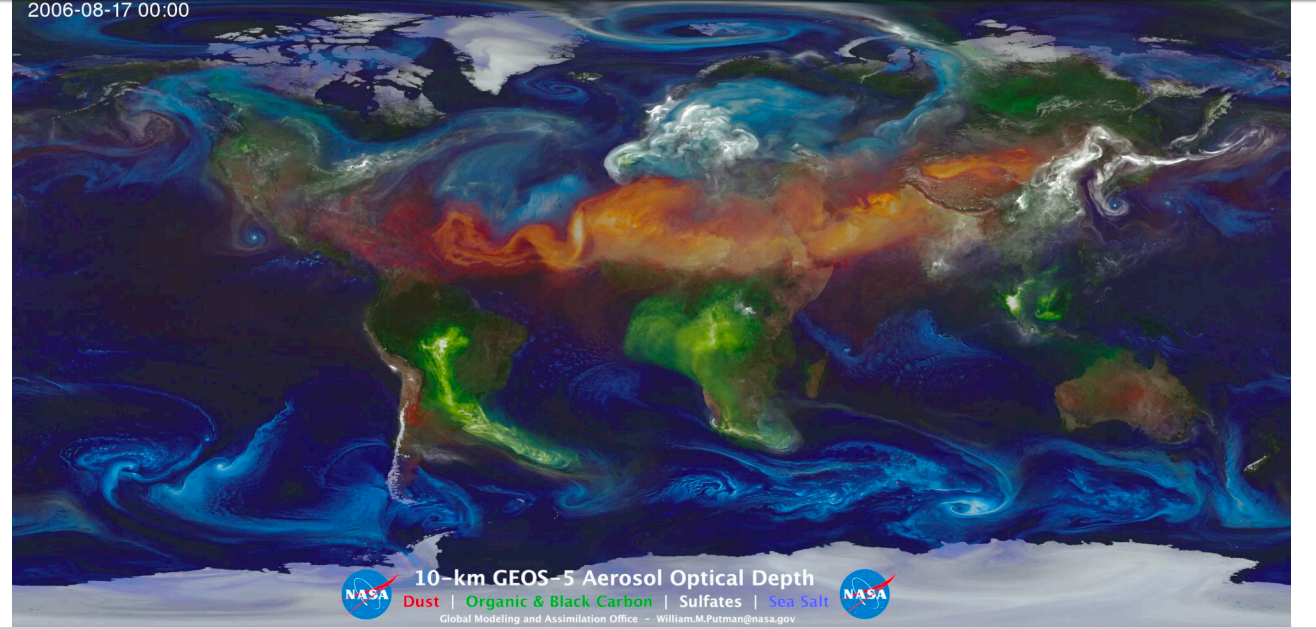
\includegraphics[scale = 0.2]{Navier.png}
 		\caption{Dinámica de fluidos.}
	\end{figure}
\end{frame}
